In this section we introduce the experiments that were carried throughout this work
along with the obtained results for each of them. The outline of the experiments can be
summarized as follows:

\begin{enumerate}
	\item At first, initial or baseline
	experiments are performed in order to replicate the results
	obtained in the previous work \cite{main} for both GMM and SVM classifiers.
	\item In a second stage, different parameters for the dynamic features are explored.
	Those parameters include the optimal proportions to be used when combining the
	supervectors with the dynamic features.
	\item At last, the final model is selected and it is tested against the hold-out data
\end{enumerate}

\section{Baseline Experiments}

% The current thesis and the previous work \cite{main} shares the same database,
% with the exception that
% data is split differently:
% In \cite{main}, a four-way jackknifing procedure containing all the instances is used to train
% and test the models, while in the current work a heldout set was kept separately of the development
% set. The number of Gaussian Mixtures composing each GMM is proportional to the number of
% training instances for that phone. In \cite{main}, a proportion of 1/25 computed
% beforehand over the total number of instances was used. In the current work, only 60\% of the
% total instances for a given phoneme is used to train each model, so the proportion of Mixture
% Components per number of instances was set to 1/15 to preserve the number of Gaussians of each
% model.

The initial experiments are carried out in order to replicate some of
the results obtained in \cite{main}.
By succesfully achieving this, one could assume that the models are being properly trained
and use them as baseline to build the new system.

The results to be replicated come from the comparison between GMM and SVM models.
The GMMs are obtained by adaptation of UBM-GMMs, as it was previously described in
the method section \ref{subsubsection:ubm}, and they are based on
a likelihood-ratio detection method.
The SVM model approach is the same as was used in this thesis, that it was also described
in the method section \ref{subsubsection:supervectors}.

% The next step was to compare the Adapted GMMs systems with the SVMs trained on supervectors.
% Results presented in \cite{main} shown that the SVMs systems produced an overall weighted EER
% relative reduction of 1.3\% with respect to the Adapted GMMs.

% Below is shown the comparison between the results obtained in the development set.

% with the Adapted GMMs initialized
% with KMeans and the results obtained with the SVMs system in the development set.
% The UBM-GMMs used to generate the
% supervector features for the SVM are trained using no initialization (such as KMeans) because
% it leads to better results.

Below is shown the
comparison of the results of the GMM models and
SVM models obtained in the development set during the experiment
replication (Fig. \ref{fig:gmmSupervectorsDev}).
The results are sorted in descending order according to their Kappa Coefficient.
Results show that the SVMs system produced an overall weighted EER relative reduction of 2.5\% with
respect to the Adapted GMMs, which is in line with the results obtained
in \cite{main}.

Additionally, it seems to exist some correlation between the phones with high Kappa
and those who achieved
the best results. This seems reasonable, because it may exist clearer differences
between correctly and mispronounced
utterances of the phones that produced better agreement over the transcribers.
These differences may lead the classifiers to perform better.
Among the eight phones with higher Kappa values (K $>$ 0.4, which implies moderate agreement):
/$\beta$/, /$\delta$/, /$\gamma$/, /b/, /w/, /m/, /i/, /s/, only /s/ exceeds an EER of 0.3.

\begin{figure}[H]
	\centering
	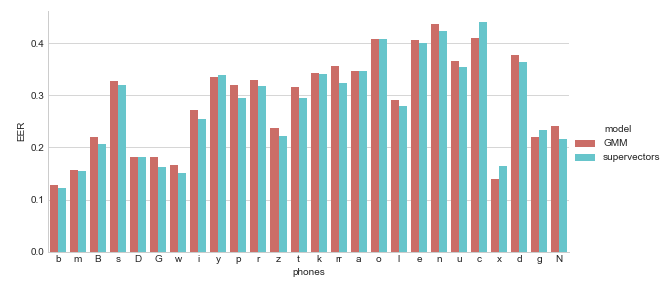
\includegraphics[width=0.8\textwidth]{files/figures/results/gmm-vs-supervectors/gmm-vs-supervectors-dev.png}
	\caption{Comparison of EER between Adapted GMMs
	and SVM trained on Supervectors for all phones obtained in the development set, sorted
	descendently by Kappa values.}
	\label{fig:gmmSupervectorsDev}
\end{figure}

At the end of the experimental phase,
the same experiment was carried out in the heldout set
leading to the results shown below
(Fig. \ref{fig:gmmSupervectorsTest}).
The models are trained using all the instances in the development set, namely, the
instances of the 4 folds.
They both have a very similar performance for each phoneme compared with the results obtained
in the development set (Fig. \ref{fig:gmmSupervectorsDev}),
from which one can deduce that both classifiers generalize well to
unobserved data. This time, however, it was the Adapted GMM model
which produced an overall weighted EER relative reduction of 0.8\% with respect to the SVMs
trained on supervectors. Even though the expected result would have been that the SVM performed
slightly better than the GMM, as it occurred in the development set,
the degradation is less than 1\% so it is still a reasonable result.

% In all the experiments
% carried out to compare the SVMs trained on supervectors and the Adapted GMMs, both classifiers
% shown a very similar performance on each phoneme.

\begin{figure}[H]
	\centering
	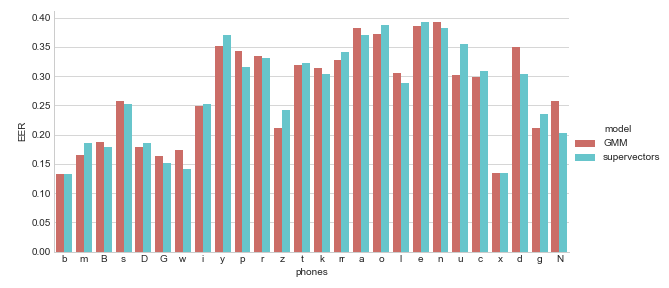
\includegraphics[width=0.8\textwidth]{files/figures/results/gmm-vs-supervectors/gmm-vs-supervectors-heldout.png}
	\caption{Comparison of EER between LLR from Adapted GMMs with K-Means initialization
	and SVM trained on Supervectors for all phones obtained in the heldout set, sorted descendently
	by Kappa values.}
	\label{fig:gmmSupervectorsTest}
\end{figure}

After the successful replication of the initial experiments, a validated SVM model based on
supervectors is obtained. This classifier is used as baseline and starting point for
the next experiments.

\section{Tunning Experiments}

Tunning experiments are carried out in order to compare both alternative
dynamic features. Features are first analysed in isolation to
determine their best possible configurations.

After that, the features generated with those configurations are combined with
the supervectors and the results of those combinations are compared to each other.

Tunning is performed in the deveopment set using 4-Fold Cross Validation. Results are
calculated only for the phones with high Kappa coefficients by averaging them.
Only these phones are considered in the process because they are the most reliable ones.

The most important parameter to be fitted is the number of coefficients to be used
for both methods. This parameter is phone-independent, that is to say, it is shared
among all the phones. This helps to keep
the models simple by reducing the number of phone-dependent configuration parameters.

\subsection{Legendre Best System}

Tunning the best Legendre configuration involves the analysis of three different
features or parameters:

\begin{itemize}
	\item Time axis normalization between -1 and 1
	\item Inclusion of duration
	\item Lasso-Regression regularization
\end{itemize}

The objective of the Legendre tunning experiments is to find the optimum degree of the Legendre
Polynomials along with the best complementary features. Degree is varied between 0 and 6,
because polynomials with
higher degrees run the risk of overfit to training instances by modeling very specific
details which are not generalizable.


\begin{figure}[H]
	\centering
	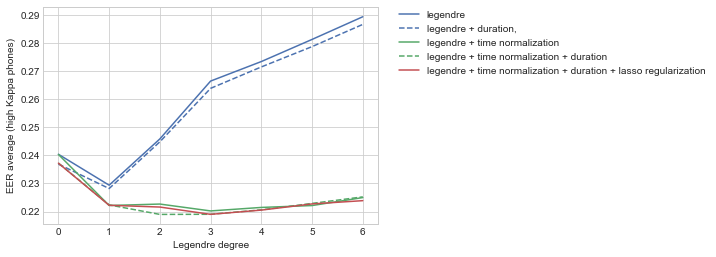
\includegraphics[width=1.0\textwidth]{files/figures/results/legendre-dct/legendre-tunning.png}
	\caption{EER average over phones with high Kappa for different
	degrees of Legendre Polynomials obtained in
	the development set. Additional configurations are also studied along with the degree and
	represented by different curves: time normalization, appending the duration and applying
	Lasso Regression.}
	\label{fig:legendreTunning}
\end{figure}

Time normalization before approximating the
MFCCs turns out to be an essential property for the Legendre Polynomials, evidenced by a
considerable reduction of the EER average (gap between the blue and green curves). At the same
time, appending the duration to the features produces a slight improvement in the performance.
Lasso Regularization, however, does not contribute to reduce the average EER.
Results show that the optimal configuration is to model the dynamics of the temporal dependencies
using Legendre Polynomials of degree 2,
along with normalizing the time axis and appending the duration of the
phone utterances to the features.

\subsection{DCT Best System and Comparison Between Features}

Analogous to Legendre, the objective of the DCT tunning experiments is to find the optimum
number of coefficients of DCT to approximate the dynamics of the temporal dependencies.
In the DCT case, the only additional parameter to be determined is whether or not appending the
duration to the DCT coefficients.

As in the Legendre optimal configuration, DCT tunning experiments also shows that appending the
duration to the coefficients produces a slight reduction in the averaged EER (around 1\%
relative).

A comparative plot between the variation of the EER as function of the number of coefficients
for both dynamic features is shown below in Fig. \ref{fig:legendreVsDCT}.
The additional parameters are fixed according to their optimal configuration
for both techinques:
Normalizing the time axis and appending the duration for Legendre (without Lasso Regularization),
and appending the duration for DCT. The degree of the Legendre Polynomials is mapped to
the number of coefficients in the \textit{x-axis} to allow the comparison:
the 0 degree Legendre Polynomial is mapped to 1 coefficient, the 1 degree Legendre Polynomial
is mapped to 2 coefficients, and so on.

\begin{figure}[H]
	\centering
	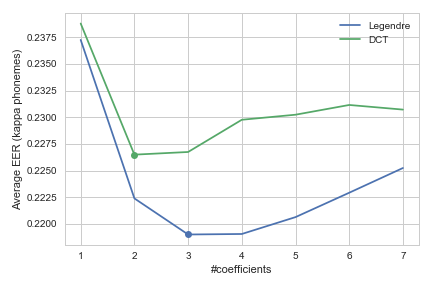
\includegraphics[width=0.5\textwidth]{files/figures/results/legendre-dct/legendre-dct-coefficients.png}
	\caption{EER average over phones with high Kappa as function of the number of coefficients
	for both Legendre Polynomials and DCT obtained in the development set.}
	\label{fig:legendreVsDCT}
\end{figure}

A dot is placed on each curve showing the optimal number of coefficients for both techniques.
As it is known from Fig. \ref{fig:legendreTunning},
the optimal number of coefficients for the
Legendre Polynomials is 3 (Polynomials of degree 2). Polynomials with 4 coefficients performs
almost as well as polynomials with 3 coefficients, but it is always preferable to keep the
model as simple as possible. On the other hand, the optimal number of coefficients for DCT is 2.

The results show that when the analysis is done in isolation (in absence of the supervectors
features), Legendre Polynomials lead to a better performance, generating a relative reduction
of the average EER of 3.3\% compared with DCT.

\subsection{Dynamic Features and Supervectors Combination Comparison}

Even though the SVM based solely on Legendre performs better than the SVM based solely on
DCT, a new experiment is carried out in order to determine which
dynamic feature integrates better
with the supervectors producing the best results.

Two types of combination are studied in the current thesis: a Features Combination and a Score
Combination. In the former, features from both sources are mixed in some proportion and
used to train a single SVM, while in the latter,
an independent SVM is trained for each feature source and
both results are combined in some proportion to generate the final results.

Again, the experiment is scoped to phones with high Kappa values.
Proportions to be used when combining the features and the scores are kept phone-dependent.
The objective is thus to compute two optimal proportions for each phone:
one for the features combinations and the other one for the score combination.

During the experiment, proportions of the dynamic features with respect to supervectors
are varied between 0 and 1 with steps of 0.1.
In other words, the explored interval is
\mbox{[0.0, 0.1, 0.2 \ldots 1.0]}.
It is worth noting that choosing
a proportion of 0.0 of the dynamic
features with respect to supervectors leads to not considering the dynamic features at all.

% both ends of the interval corresponds to use only
% a feature source and not using the other source at all. A proportion of 0.0 of the dynamic
% features with respect to supervectors leads to not considering the dynamic features at all
% while a proportion of 1.0 leads to not using the supervectors features at all.
% In the case of the Features Combination, an extra exploration is done in the interval
% [0.0 - 0.1], because achieving an optimal feature combination may have required a more
% refined granularity in the proportions. No significant gains, however, were observed
% when zooming in in the interval [0.0 - 0.1].

In the Features Combination experiment,
the optimal proportion for the majority of the phones
for both Legendre and DCT approaches turns out to be 0.1.
% For the Features Combination case, the optimal proportion for the majority of the phonemes
% for both Legendre and DCT approaches is 0.1.
There are also some phones such as
$/\gamma/$ and $/b/$ where the best proportion is 0.0.
This can be interpreted as that
no proportion produces an improvement when combining the dynamic features with the supervectors.

On the other hand, in the Score Combination experiment, the optimal proportions for
the results of the different phones are more scattered along the whole interval [0.0 - 1.0]
for both Legendre and
DCT. Again, there are also some phones for which the optimal proportion is 0.0, but they are
considerable fewer than in the features combination case.

For both combination types, the DCT features yield better results than the Legendre features,
though the results for both features are very close to each other (around 1\% of relative
difference), as it is shown in Table \ref{table:legendreVsDCTCombinations}.

~

\begin{table}[h]
	\renewcommand{\arraystretch}{1.5}
	\begin{center}
	    \begin{tabular}{ | c | c | c | }
	    \hline
	    & Legendre + Supervectors & DCT + Supervectors \\ \hline
	    EER Features Combination (Avg) & 0.188 & 0.187 \\ \hline
	    EER Score Combination (Avg) & 0.189  & 0.187 \\ \hline
	    \end{tabular}
	    \caption{EER average over phones with high Kappa using the best proportions for
	    both Dynamic Features and combination approaches, obtained in the development set.}
	    \label{table:legendreVsDCTCombinations}
	\end{center}
\end{table}

At this point, the DCT features are chosen as the Dynamic Features to be combined with the
supervectors when training the final models, and for each of the remaining phones with
low Kappa values the phone-dependent proportions are computed.

\section{Final Models Validation}

The final experiments are carried out in order
to determine if there is a real gain when combining
supervectors with DCT features compared with training an SVM based only on supervectors.
Additionally, we are interested to see if any of both fusion systems is better
than the other one. The three systems to be compared are then:

\begin{itemize}
	\item SVM trained only on supervectors, which is used as the baseline system.
	\item SVM trained on the features combination of DCT and supervectors (using the best features combination proportions obtained in the tunning phase).
	\item System based on the score combination of an SVM trained
	only on supervectors and an SVM trained
	only on DCT features (using the best score combination proportions obtained in the tunning phase).
\end{itemize}

An initial experiment is performed in the development set
followed by a second experiment, where
the final models are tested against the heldout data.
% by testing the final models using at first
% the development data and then testing them against the heldout data.
The relative gains of the final models
are calculated using the SVM trained only on supervectors as baseline system.

% with respect to the baseline system: SVM trained on supervectors
% features only.

Unlike the tunning phase, where the experimentation is driven by the results obtained
over the phones with higher kappa values, a new criteria is used for the model validation.
A McNemar test is performed as previous step to scope the analysis
to a subset of phones with statistically significant results in the development
data (\textit{p-value} $<$ 0.05).
McNemar, which is described in Method Section \ref{subsection:mcnemar},
is used to estimate the confidence that a final model is different from
the baseline model by using the paired nominal results of both classifiers.

% McNemar is used to estimate confidence of the two classifiers being actually different
% using the paired nominal results of both classifiers (\ref{subsection:mcnemar}).
% The McNemar test is run using the SVM
% trained only on supervectors as baseline of the comparison.

\subsection{Development Results}

The comparison of the three systems
in the development set is carried out using a 4-Fold Cross Validation
approach. The results for each of
the systems are derived from the combination of the
results obtained in each of the folds.
In addition, McNemar's test is computed to determine if the
results are statistically significant.

The results for all the phones are summarized in the left side of both tables
\ref{tab:featuresCombinationAppendixTable} and \ref{tab:scoreCombinationAppendixTable}
of the Appendix A Section. Rows with grey background corresponds to the phones for which
the McNemar's test gives significant results in the development set, which are the
phones of interest. Those are:

\begin{itemize}
	\item /s/, /y/, /e/, /o/, /l/, /n/, /m/ in Features Combination
	\item /s/, /y/, /e/, /o/, /l/, /z/, /n/, /m/, /rr/, /t/ in Score Combination
\end{itemize}

The relative gains for the phones mentioned above are summarized in
Fig. \ref{fig:fusionMcnemarDev}.
A visual reference (*) is added on top of each bar to indicate if that value
is statistically significant.
It is worth noting that phones with statistically significant results in the Features
Combination experiment are a subset of the phone with statistically significant results in the
Score Combination experiment. For that reason, all the bars of the Score Combination experiment
have a visual reference (*) on top, but some of the bars of the Features Combination do not
have it.

% even though the barplots includes
% the results for the ten statistically significant phonemes of the Score Combination,
% additional marks (*) and (**) are included for the Features Combination bars to
% point out whether or not those results are significant in the Features Combination
% case.

\begin{figure}[H]
	\centering
	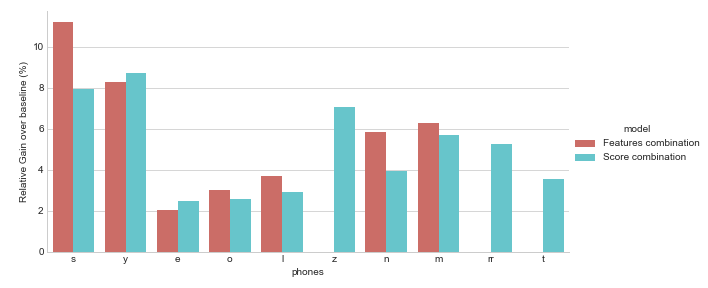
\includegraphics[width=0.8\textwidth]{files/figures/results/relatives/relatives-fusion-systems-dev-mcnemar.png}
	\caption{Comparison of relative gains over the Baseline System
	between the Features Combination systems
	and the Score Combination systems
	computed on the development set. Results are sorted descendently by McNemar's p-value.
	A visual reference (*) is added on top of the bars
	for each \textless phone, fusion type\textgreater \ pair that produces
	statistically significant results.}

	% For all the score combinations phones the results were significant in the training set,
	% whereas for the features combination phones only the phones marked with (*) were significant,
	% and those marked with (**) weren't significant.
	\label{fig:fusionMcnemarDev}
\end{figure}

\subsection{Hold-out results}

In this experiment, the three aforementioned systems are trained using all the instances of the
development set and tested against the hold-out set.

The analysis is again scoped to our phones of interest, which are those with statistically
significant results in the development set.
The obtained results for all the phones, however, is available
in the right side of both tables
\ref{tab:featuresCombinationAppendixTable} and \ref{tab:scoreCombinationAppendixTable}
of the Appendix A Section.
Even though a new McNemar test is computed on the
results obtained in the hold-out data, it does not yield statistically significant results
for our phones of interest. This can be explained by the fact that hold-out data
has around 1/4 of the data of the
development data, affecting the efectiveness of the test.

% To run the experiment against the heldout data, the models were trained using all the
% instances of the development set.

% A new McNemar test is performed for the results obtained
% in the heldout data for the same phoneme with statistically significant results in the
% development data, but this time any of them gave a significant p-value $<$ 0.05.
% This can be explained by the fact that heldout data has around 1/4 of the data of the
% development data, affecting the efectiveness of the test.

% The results are then still scoped to the phonemes with statistically significant results
% in the development experiment, and the same notation (*) and (**) is kept as a reference.

The relative gains for the phones of interest are summarized in Fig. \ref{fig:fusionMcnemarTest}.
Again, a visual reference (*) is added on top of each bar to indicate the cases were the
values obtained in the development set were statistically significant.

\begin{figure}[H]
	\centering
	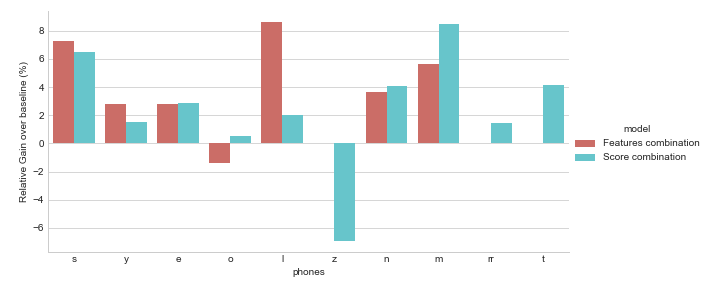
\includegraphics[width=0.9\textwidth]{files/figures/results/relatives/relative-fusion-systems-heldout-mcnemar.png}
	\caption{Comparison of relative gains over the Baseline System
	between Features Combination systems and Score Combination
	systems computed on the hold-out set for the phones of interest.
	Results are sorted descendently by their McNemar's p-value computed on the development set.
	A visual reference (*) is added on top of the bars
	for each \textless phone, fusion type\textgreater \ pair that produced
	statistically significant results in the development set.}
	\label{fig:fusionMcnemarTest}
\end{figure}

Among the phones that were statistically significant in the Score Combination
experiment carried out in the development set, only 'z' degrades its performance compared
with the baseline system around a 6\% relative. Among the
remaining phones, some reduce its gain compared with the development set (such as
/y/ from 8\% to less than 2\% and /rr/ from almost 6\% to less than 2\%). Others such
as /m/ improves its performance from 6\% to more than 8\%.

On the other hand, among all the phones that were statistically significant in the
Features Combination experiment carried out in the development set, only /o/ degrades
its performance and in a slightly way. The plots also show a degradation of the /rr/
performance, but /rr/ did not yield statistically significant
in the Features Combination
experiment carried out in the development set.
As in the case of the Score Combination, among the remaining phones
there are cases where both improvements
and degradations of the performance are observed.

% One important aspect to be analysed in the next section is whether or not the Score Combination
% of the results leads to a more robust classifier than the Features Combination technique.


